\begin{exercice}[Plusieurs triangles]
\begin{itemize}
 \item $RAT$ est un triangle tel que $RA = 7$ cm ; $TA = 6$ cm et $\widehat{RAT} = 40^\circ$ ;
 \item $RIT$ est un triangle tel que $\widehat{RTI} = 57^\circ$ ; $\widehat{TRI} = 82^\circ$.
 \end{itemize}
\vspace{-0.5cm}
Dans chaque cas fais un croquis des triangles puis construis-les. Que remarques-tu ? 
\end{exercice}


\begin{exercice}[Triangles et cercle]
Construis un triangle $LAC$ isocèle en $C$ tel que $LA = 3$ cm et $LC = 5$ cm :
\begin{enumerate}
 \item Trace le cercle de centre $C$ passant par $A$. Que constates‑tu ?
 \item Construis si possible un triangle $ABC$ équilatéral tel que $B$ appartienne à ce cercle.
 \end{enumerate}
\end{exercice}


\begin{exercice}[À partir d'un programme]
Réalise la figure correspondant au programme de construction ci‑dessous :
\begin{itemize}
 \item Trace un triangle $ABC$ rectangle en $B$ avec $AB = 4$ cm et $BC = 6$ cm ;
 \item Trace le rectangle $ACDE$ avec $AE = 5$ cm de telle sorte que $B$ soit un point extérieur à $ACDE$ ;
 \item Trace la droite $d$ perpendiculaire à $(AB)$ passant par $A$ ;
 \item Trace $d'$ la médiatrice de $[DE]$ ;
 \item Place $F$ le point d'intersection de $d$ et $d'$ ;
 \item Trace la droite $d''$ parallèle à $(AC)$ passant par $B$.
 \end{itemize}
Que peux‑tu dire des droites $d'$ et $d''$ ? (Justifie)
\end{exercice}


\begin{exercice}[Avec des médiatrices]
Construis le triangle $ABC$ tel que $AB = 8$ cm ; $AC = 4$ cm et $BC = 6$ cm. Trace $d_1$ la médiatrice de $[AB]$ et $d_2$ la médiatrice de $[BC]$. Les droites $d_1$ et $d_2$ sont sécantes en $O$. Trace $d_3$ la parallèle à $(BC)$ passant par $O$. Que peux‑tu dire des droites $d_2$ et $d_3$ ?
\end{exercice}


\begin{exercice}[Avec le périmètre et les angles]
On veut tracer un triangle tel que son périmètre mesure 16 cm et deux de ses angles mesurent $64^\circ$ et $46^\circ$ :
\begin{enumerate}
 \item Effectue un croquis de ce triangle et calcule la mesure de son troisième angle ;
 \item Trace un segment $[DE]$ mesurant 16 cm et place $A$ tel que : $\widehat{ADE} = 32^\circ$ et $\widehat{AED} = 23^\circ$ (on a pris les moitiés de $64^\circ$ et $46^\circ$) ;
 \item Place un point $B$ sur le segment $[DE]$ à égale distance de $A$ et de $D$ puis un point $C$ sur le segment $[DE]$ à égale distance de $A$ et de $E$. Indique la nature des triangles $ABD$ et $ACE$ ;
 \item Mesure les angles des triangles $ABD$ et $ACE$ ;
 \item Compare le périmètre et les angles du triangle $ABC$ avec ceux du triangle cherché ;
 \item Trace un triangle $RST$ de périmètre 20 cm tel que $\widehat{RST} = 36^\circ$ et $\widehat{STR} = 68^\circ$.
 \end{enumerate}
\end{exercice}


\begin{exercice}[Un joli cercle d'amis]
\begin{enumerate}
 \item Kévin et Nicolas ont tous les deux leur arbre fétiche sous lequel ils aiment se reposer. Mais ils aiment aussi faire la course en partant chacun de leur arbre. Pour que la course soit équitable, il faut que l'arrivée soit située à la même distance des deux arbres.
 \begin{itemize}
  \item Sur ton cahier, place deux points $K$ et $N$ (distant de 4 cm) pour représenter les arbres de Kévin et de Nicolas. Construis ensuite un point à égale distance des deux arbres $K$ et $N$ et places-y un drapeau.
  \item Où placer l'arrivée pour que la course soit la plus courte possible ?
  \item Si Kévin et Nicolas veulent une course plus longue, où peuvent-ils encore planter le drapeau ? Quel est l'ensemble des points possibles pour l'arrivée ? Trace-le en bleu. 
  \end{itemize}
 \item Gabin a aussi son arbre et il aimerait bien jouer avec Nicolas au même jeu. Sur ton cahier, place un point $G$, comme sur la figure ci-dessous représentant l'arbre de Gabin.
 \begin{center} 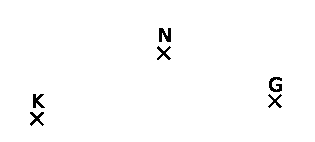
\includegraphics[width=4cm]{pointsKNG} \end{center}
 \begin{itemize}
  \item Trace \textbf{\textcolor{B2}{en rouge}} l'ensemble des points équidistants des arbres de Gabin et de Nicolas.
  \item Mais Kévin, désormais, s'ennuie. Il propose : « Organisons une course à trois ! ». Où peuvent-ils planter le drapeau ? Pourquoi ? 
  \item Yann n'a pas d'arbre à lui mais veut aussi courir. Nicolas dit : « Si tu veux jouer, ton arbre doit être aussi loin du drapeau que les nôtres ! » Place plusieurs points où pourrait être l'arbre de Yann. Où semblent se situer ces points ? 
  \item Trace l'ensemble des points où pourrait être l'arbre de Yann.
  \end{itemize}
 \end{enumerate}
\end{exercice}
